\section{Θεωρία Γράφων}
\selectlanguage{english}
\subsection{Ιστορική Αναδρομή}
\begin{figure}[ht]
    \begin{minipage}[c]{.46\linewidth}
        \centering
        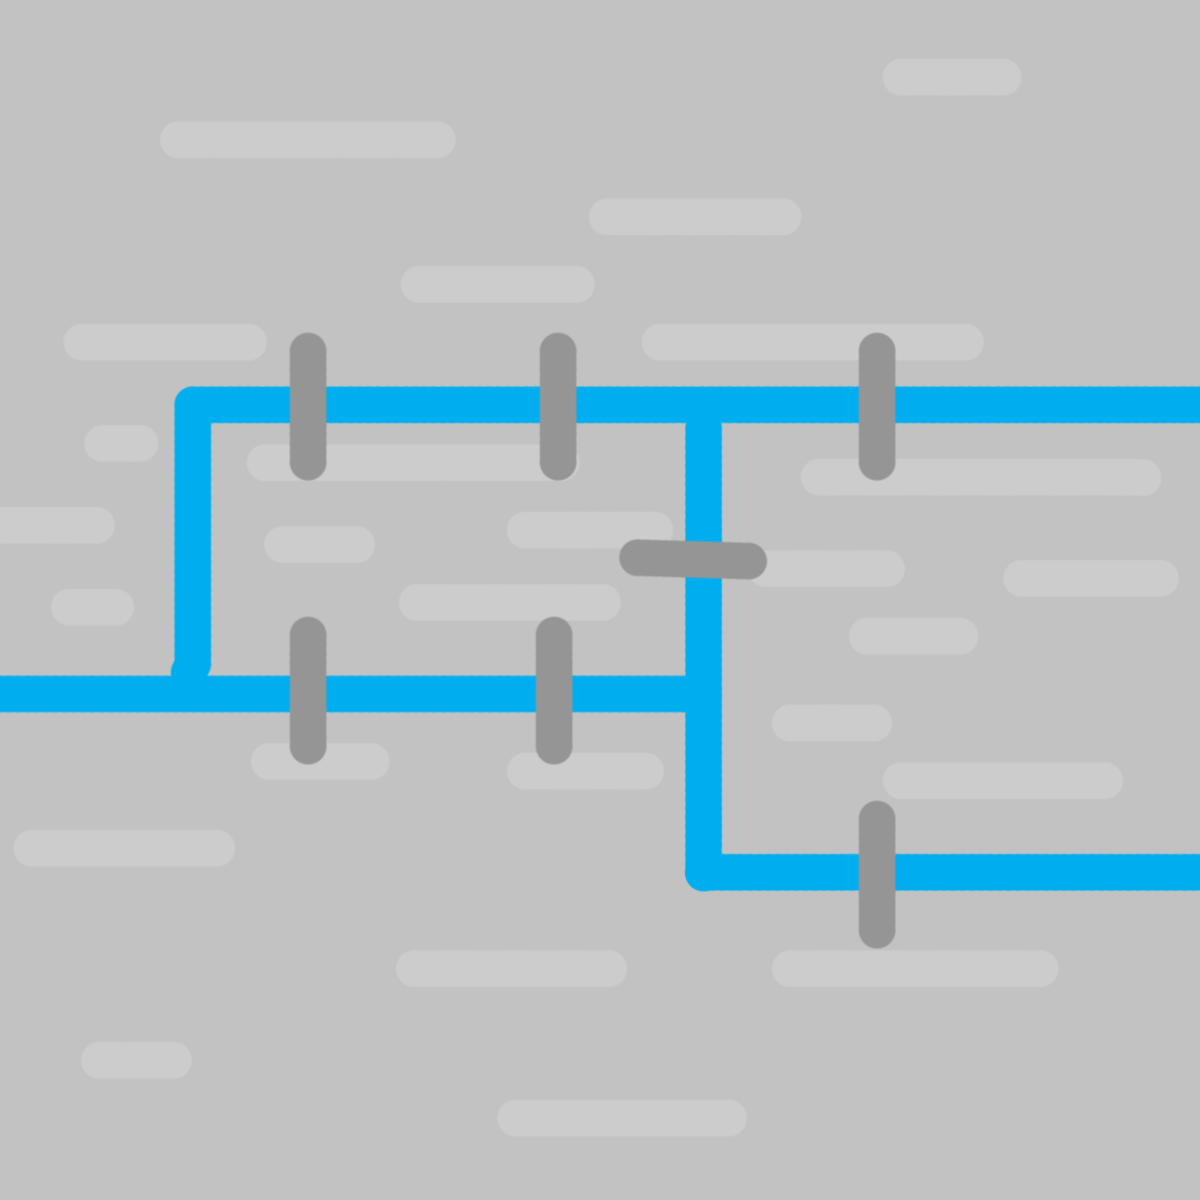
\includegraphics[scale=0.15]{2947_thesis/pictures/konigsberg.png}
        \caption{Προσομοίωση Königsberg.}
        \label{1}
    \end{minipage}
    \hfill%
    \begin{minipage}[c]{.46\linewidth}
        \centering
        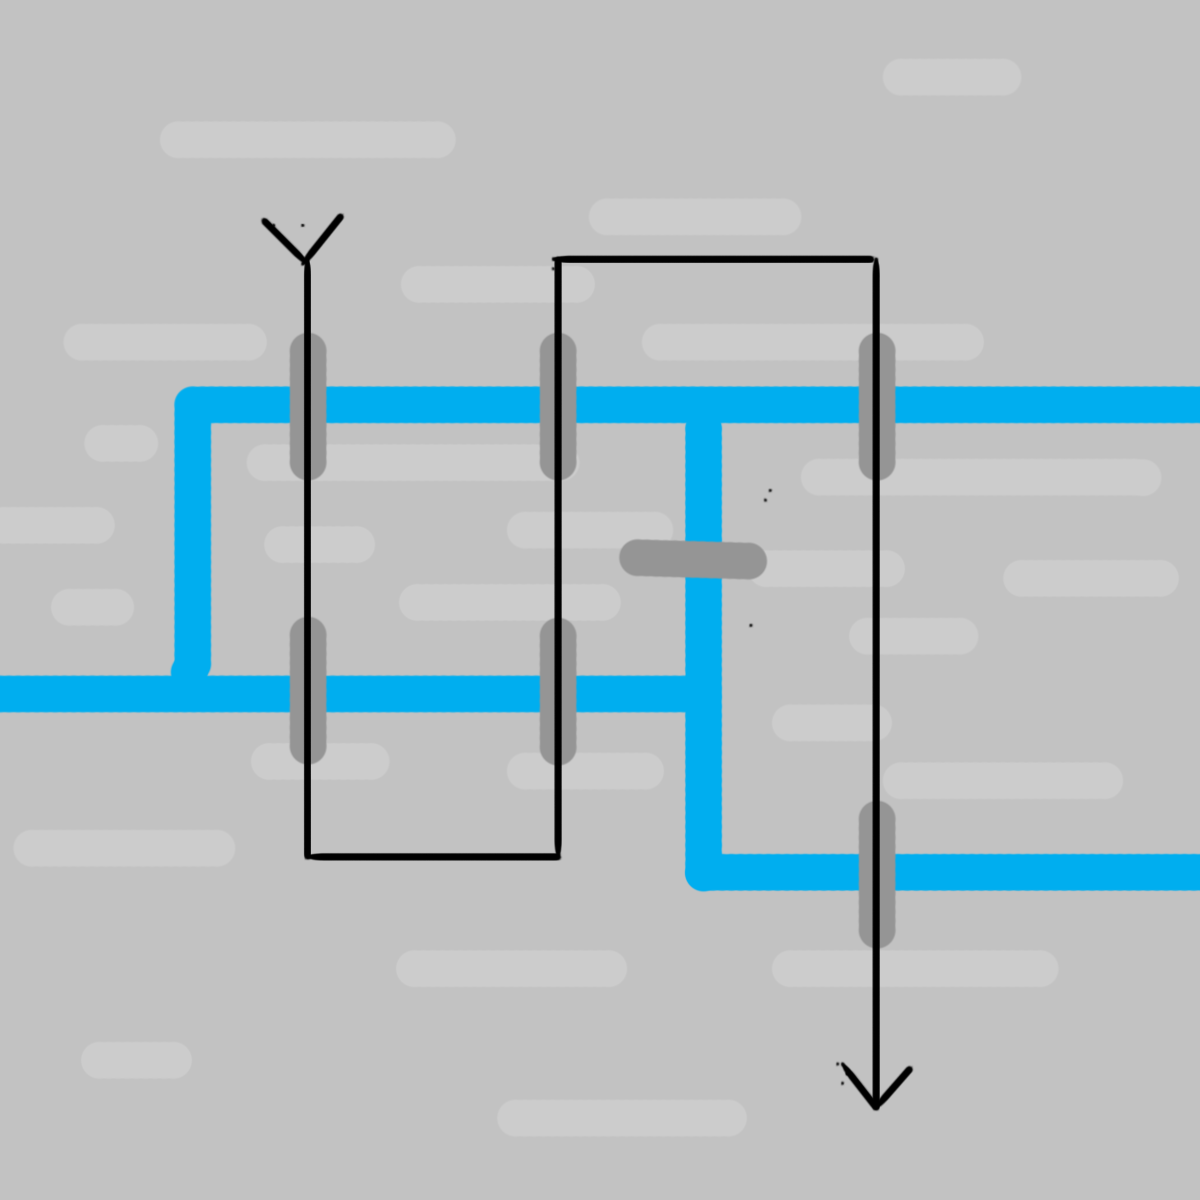
\includegraphics[scale=0.15]{2947_thesis/pictures/konigsbergEx.png} 
        \caption{Παράδειγμα διάσχισης γεφυρών}
        \label{2}
    \end{minipage}
\end{figure}
\begin{figure}[ht]
    \begin{minipage}[c]{.46\linewidth}
        \centering
        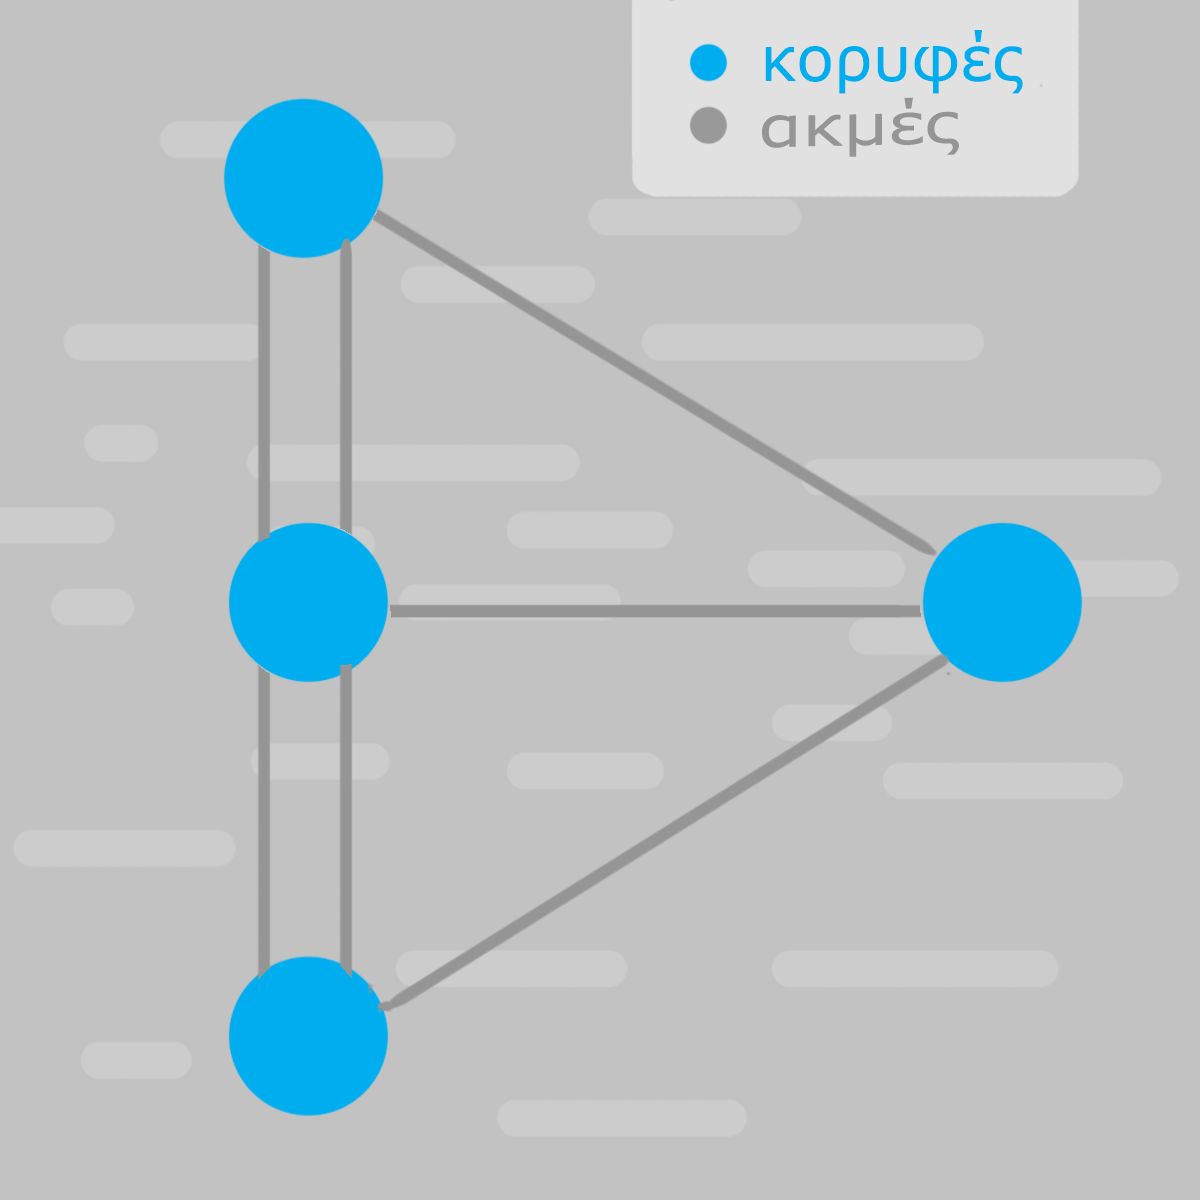
\includegraphics[scale=0.15]{2947_thesis/pictures/konigsberGraph.png}
        \caption{Königsberg ως γράφος.}
        \label{3}
    \end{minipage}
    \hfill%
    \begin{minipage}[c]{.46\linewidth}
        \centering
        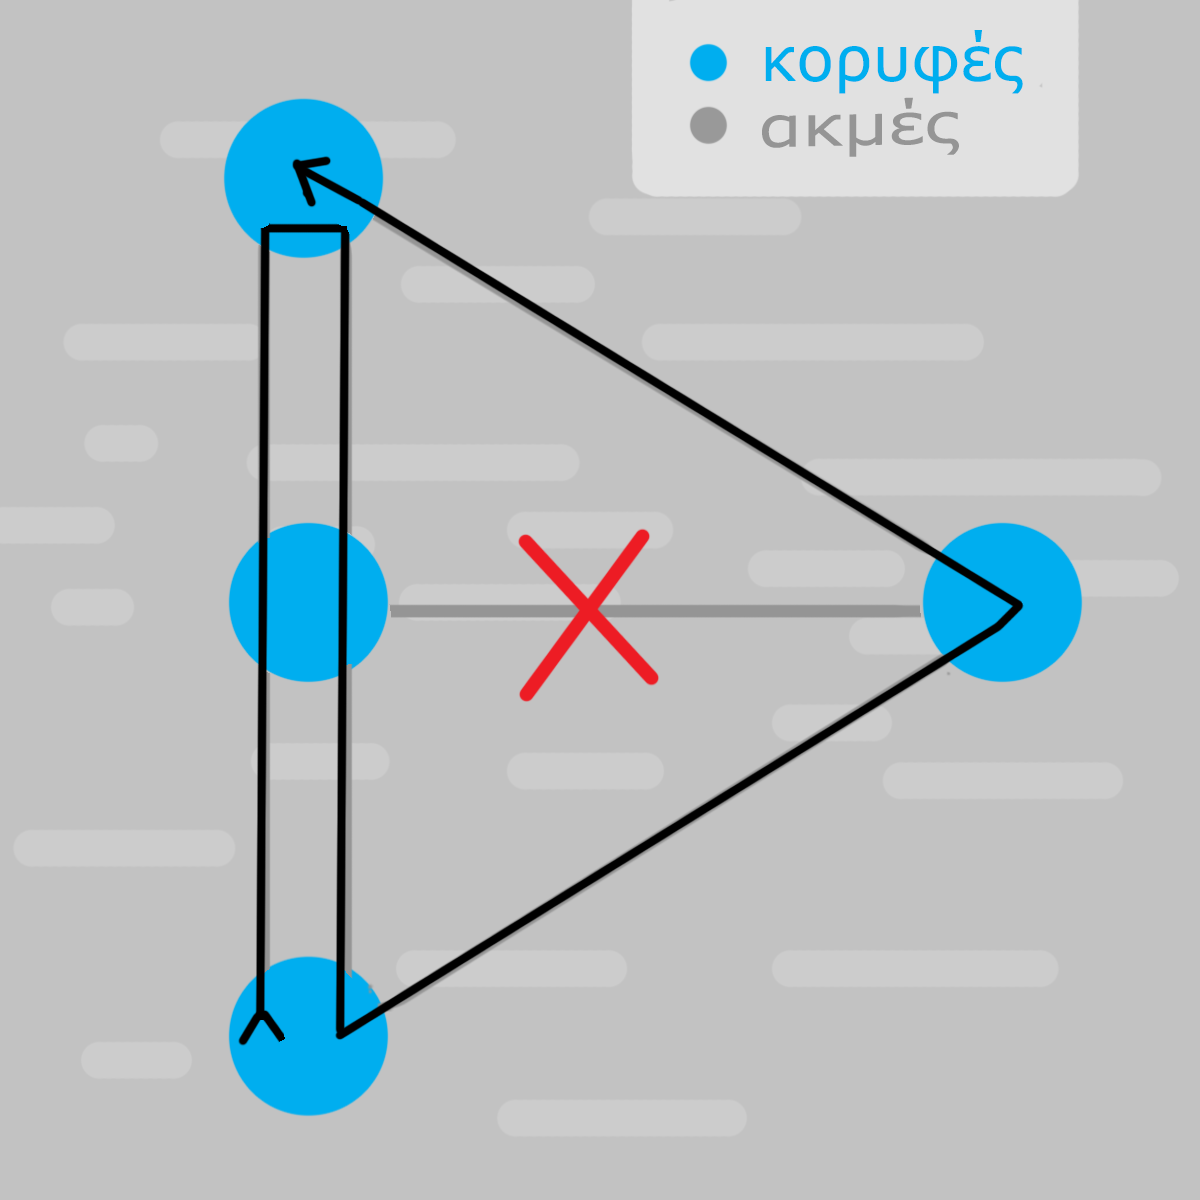
\includegraphics[scale=0.15]{2947_thesis/pictures/konigsbergEuler.png}
        \caption{Διαδρομή Όιλερ.}
        \label{4}
    \end{minipage}
\end{figure} 
Η ανάπτυξη της θεωρίας γράφων (graph theory) ξεκίνησε τον 18ο αιώνα και πιο συγκεκριμένα το 1736 στην πόλη Königsberg της Πρωσίας. Σήμερα είναι το Ρωσικό Kaliningrad (μεταξύ Λιθουανίας και Πολωνίας στη Βαλτική) \cite{manwlopoulos2014thewria}. Η πόλη ήταν χωρισμένη σε 4 τμήματα από τον ποταμό Pregel και χρησιμοποιούνταν 7 γέφυρες για να γίνεται εφικτή η διέλευση των κατοίκων στα διάφορα τμήματά της [Figure \ref{1}]. Όταν ο Ελβετός μαθηματικός Λέοναρντ Όιλερ (Leonard Euler) αναρωτήθηκε αν είναι εφικτό να διασχίσει κάποιος τις γέφυρες της πόλης με βασικό περιορισμό να διασχιστούν όλες οι γέφυρες μόνο μία φορά (Πρόβλημα των 7 γεφυρών του Königsberg )[Figure \ref{2}], έτσι ένας νέος κλάδος των διακριτών μαθηματικών γεννήθηκε, γνωστός και ως θεωρία γράφων. Ο Όιλερ απέδειξε ότι δεν υπάρχει τέτοια διαδρομή μέσω της χρήσης γράφων και κατά συνέπεια το πρόβλημα δεν έχει λύση. Αυτή η απόδειξη απέκτησε αξία όταν ο Όιλερ την εφάρμοσε και σε άλλα προβλήματα γράφων και γενίκευσε την βασική ιδέα. 

Ένα μονοπάτι (path) ονομάζεται μονοπάτι Όιλερ (Eulerian path or Eulerian trail) όταν μπορούμε να επισκεφτούμε κάθε περιοχή-κορυφή (vertice) διασχίζοντας την κάθε γέφυρα-ακμή (edge) μόνο μία φορά (και ονομάζεται κυκλική αν καταλήγουμε εκεί που ξεκινήσαμε), αν υπάρχει ένα τέτοιο μονοπάτι σε ένα γράφο τότε αυτός ο γράφος ονομάζεται γράφος Όιλερ (Eulerian graph). \cite{ntenisiwtis2023thewria}. Στο σχήμα [Figure \ref{3}] που αντιπροσωπεύει την πόλη του Königsberg σε μορφή γράφου δεν υπάρχει μια τέτοια διαδρομή. Για να γίνει αυτό πρέπει να αφαιρέσουμε μία γέφυρα-ακμή [Figure \ref{4}]. Παρατηρήθηκε από τον Όιλερ ότι όλες οι κορυφές πρέπει να έχουν άρτιο βαθμό εκτός από αυτές που ξεκινά και τελειώνει η διαδρομή, εκτός κι αν η διαδρομή είναι κυκλική. Πιο συγκεκριμένα, ένας συνδεδεμένος γράφος $Graph(Vertices,Edges)$ είναι γράφος Όιλερ αν και μόνο αν δεν έχει κορυφές (vertices) περιττού βαθμού. \cite{bondy1976usr}


\subsection{Εισαγωγή στην Θεωρία Γράφων}

Στην ουσία, ένας γράφος (graph) είναι διάσπαρτα σημεία-κορυφές (vertices) που ενώνονται με γραμμές-ακμές (edges). Γράφους μπορούμε να συναντήσουμε σε διάφορα προβλήματα της καθημερινότητας όπως δίκτυα υποδομών (πχ δίκτυο ύδρευσης), προβλήματα χαρτογράφησης (πλοήγηση), τηλεπικοινωνιών (πχ δορυφόροι), μεταφορών (πχ σιδηρόδρομοι) , και άλλα \cite{manwlopoulos2014thewria}. Η θεωρία γράφων είναι ένας σημαντικός τομέας των μαθηματικών γιατί πέρα από το γεγονός ότι με χρήση αυτής μπορούμε να μοντελοποιήσουμε εύκολα προβλήματα της καθημερινότητας μας σε τομείς που αναφέρθηκαν παραπάνω, μπορούμε επίσης να αναπτύξουμε αλγόριθμους που λύνουν προβλήματα με χρήση γράφων. Παράδειγμα αυτού είναι και ο αλγόριθμος αποικίας των μυρμηγκιών (ACO) που θα αναλύσουμε σε αυτήν την πτυχιακή εργασία.

\subsection{Βασικοί Ορισμοί και έννοιες}
Για να γίνουν κατανοητά όσα θα αναφερθούν στην παρακάτω εργασία είναι απαραίτητο να παρουσιαστεί το θεωρητικό υπόβαθρο πάνω στο οποίο είναι βασισμένοι οι αλγόριθμοι βελτιστοποίησης. Για πιο αναλυτική μελέτη παραπέμπονται οι βιβλιογραφικές αναφορές που χρησιμοποιήθηκαν στο τέλος της εργασίας.

Ένας γράφος είναι μία μαθηματική δομή που ορίζεται με αυστηρό τρόπο μέσω δύο συνόλων: το σύνολο κόμβων (ή κορυφών, vertices) και το σύνολο ακμών (ή γραμμών, edges) που συνδέουν ζεύγη κορυφών μεταξύ τους και χρησιμοποιείται για την αναπαράσταση πληροφορίας σχετικά με συνδεσμολογία \cite{ntenisiwtis2023thewria}. Όταν δύο κορυφές είναι συνδεδεμένες, δηλαδή ενώνονται με τουλάχιστον μία ακμή ονομάζονται γειτονικές (adjacent vertices) (για παράδειγμα στο [Figure \ref{5}] η κορυφή "Α" και η κορυφή "Β" είναι γειτονικές), αντίστοιχα δύο ακμές που καταλήγουν σε ίδια κορυφή ονομάζονται προσπίπτουσες (incident edges) της κορυφής αυτής. Το πλήθος των ακμών που προσπίπτουν σε μία κορυφή καλείτε βαθμός (degree) ή αξία (valency) της κορυφής αυτής. Τάξη (order) ενός γράφου καλούμε το πλήθος των κορυφών που έχει (για παράδειγμα στο [Figure \ref{5}] η κορυφή "Ε" είναι τέταρτου βαθμού και ο γράφος είναι έκτης τάξης) . Ένας γράφος μπορεί να είναι είτε κατευθυνόμενος (directed graph) όταν οι ακμές έχουν κατεύθυνση από μία κορυφή προς μία άλλη [Figure \ref{6}], είτε μη-κατευθυνόμενος (undirected graph) όταν οι ακμές δεν έχουν κατεύθυνση και μπορούν να πηγαίνουν προς οπουδήποτε μεταξύ των κόμβων [Figure \ref{5}]. \cite{gkertsis2023thewria} \footnote{για περαιτέρω μελέτη: Directed and Undirected Graphs από mathworks\\ link: \url{https://www.mathworks.com/help/matlab/math/directed-and-undirected-graphs.html}}

Στις ακμές ενός γράφου μπορεί να γίνει επισύναψη βάρους (weight), το οποίο αντιπροσωπεύει το κόστος, την απόσταση ή άλλες χρήσιμες πληροφορίες που συνδέονται με τις σχέσεις μεταξύ των κορυφών. Ένας γράφος που οι ακμές του έχουν συσχετιστεί με έναν αριθμό ονομάζονται γράφος με βάρη (weighted graph). Τα βάρη μπορούν να χρησιμοποιηθούν για την εκτέλεση αλγορίθμων βελτιστοποίησης και την αναζήτηση των βέλτιστων μονοπατιών σε γράφο \cite{ntenisiwtis2023thewria}, \cite{gkertsis2023thewria}. Στον αλγόριθμο που θα αναλυθεί σε αυτήν την πτυχιακή εργασία τα βάρη αντιπροσωπεύουν την απόσταση της διαδρομής ή το επίπεδο της φερομόνης (θα αναλυθεί σε επόμενο κεφάλαιο).



\begin{figure}[ht]
    \begin{minipage}[c]{.46\linewidth}
        \centering
        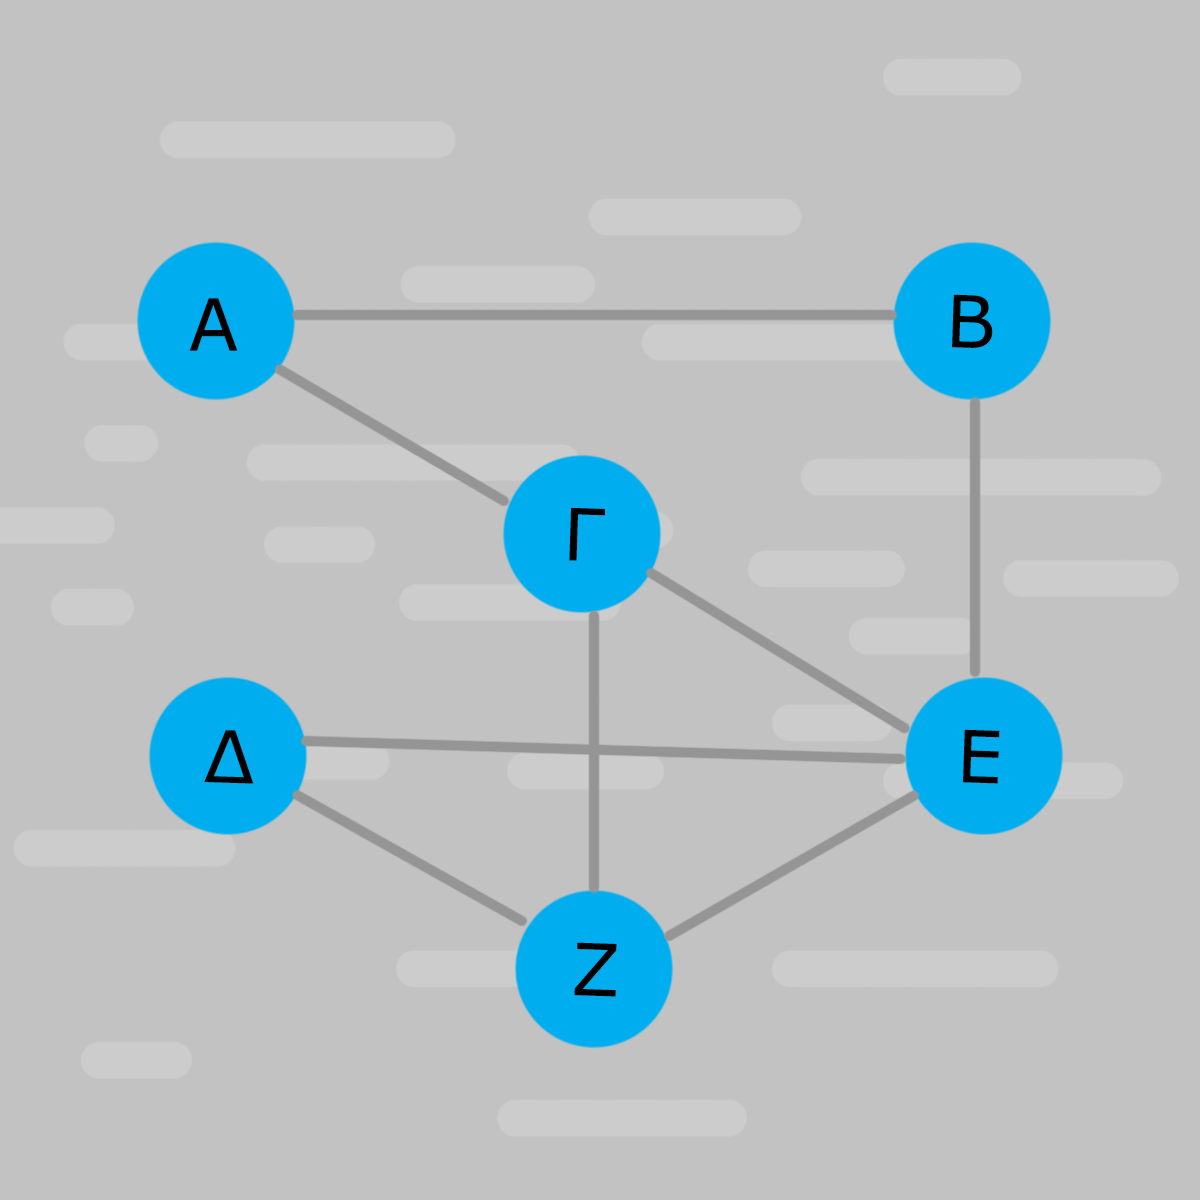
\includegraphics[scale=0.15]{2947_thesis/pictures/undirected.png}
        \caption{Μη κατευθυνόμενος γράφος.}
        \label{5}
    \end{minipage}
    \hfill%
    \begin{minipage}[c]{.46\linewidth}
        \centering
        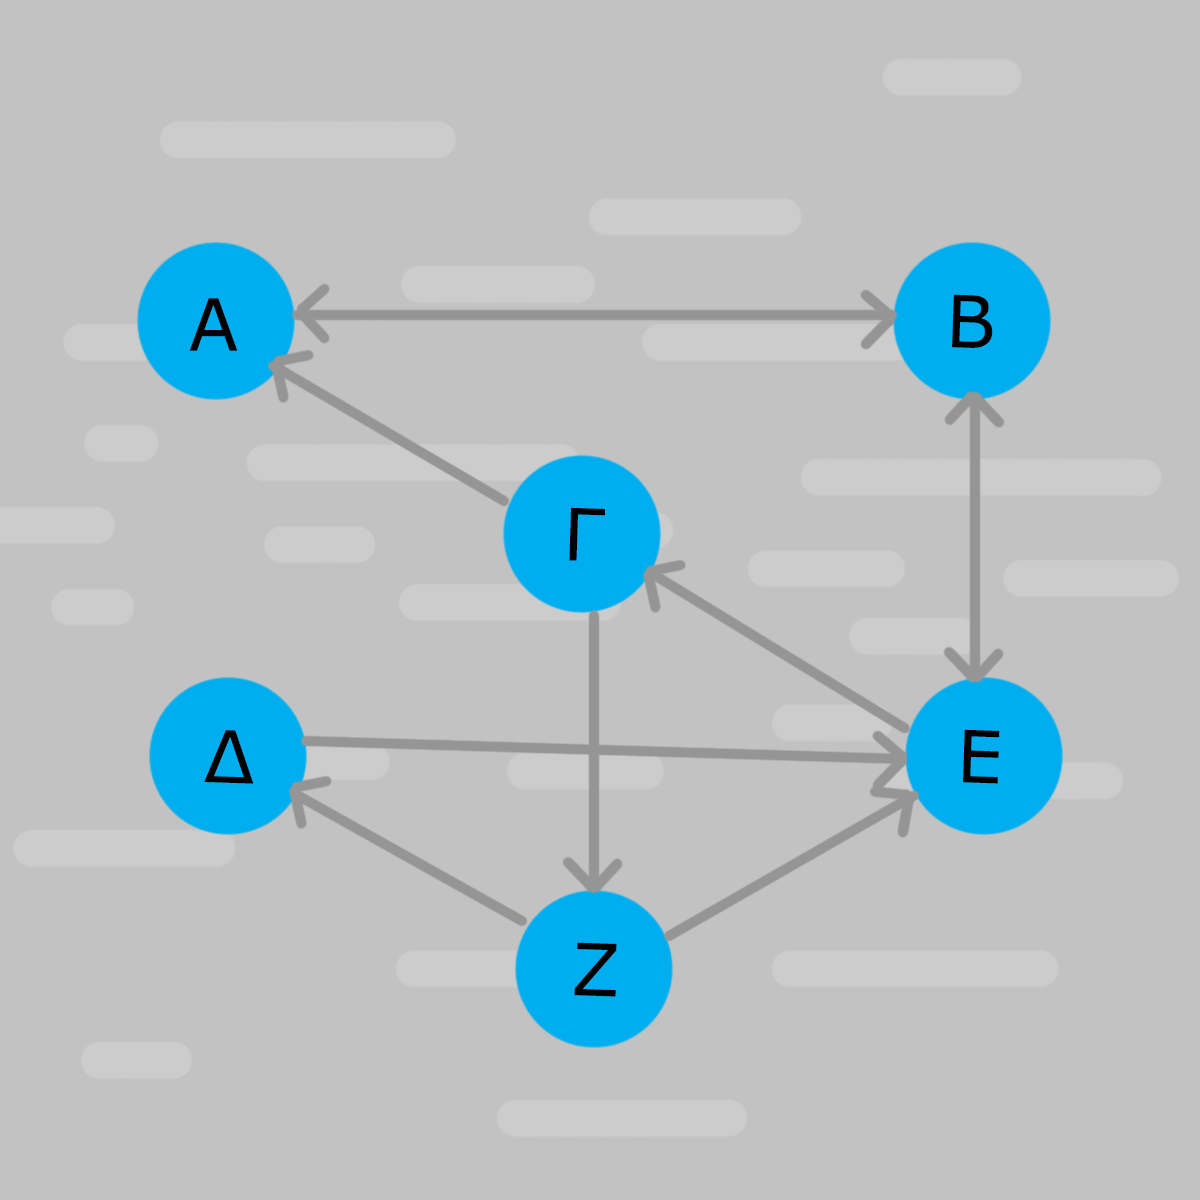
\includegraphics[scale=0.15]{2947_thesis/pictures/directed.png} 
        \caption{Κατευθυνόμενος γράφος.}
        \label{6}
    \end{minipage}
\end{figure}

\subsection{Μαθηματικό υπόβαθρο}
Ένας γράφος (Graph) $G$ ορίζεται από δύο σύνολα $V(G)$ και $E(G)$. Το σύνολο $V(G)$ είναι ένα πεπερασμένο σύνολο (μη άπειρο), που περιέχει ως στοιχεία τις κορυφές (Vertices) του γράφου. Το σύνολο $E(G)$ περιέχει τις ακμές (Edges) ενός γράφου εκφρασμένες με δισύνολα δύο γειτονικών κορυφών. Έτσι, πεπερασμένος (μη - κατευθυνόμενος, undirected) γράφος, λέγεται το διατεταγμένος ζεύγος $G = (V(G), E(G))$ των πεπερασμένων συνόλων $V(G)$, $E(G)$ \cite{ntenisiwtis2023thewria}. Αν πάρουμε ως παράδειγμα τον γράφο $G$ στο [Figure \ref{7}] παρατηρούμε ότι τα σύνολα $V(G)$ και $E(G)$ έχουν ως εξής: 
\begin{itemize}
  \item $V(G)=$[$v1,v2,v3,v4$]
  \item $E(G)=$[$e1(v1,v2),e2(v1,v3),e3(v2,v3),e4(v3,v4)$] 
\end{itemize}

\begin{figure}
    \centering
    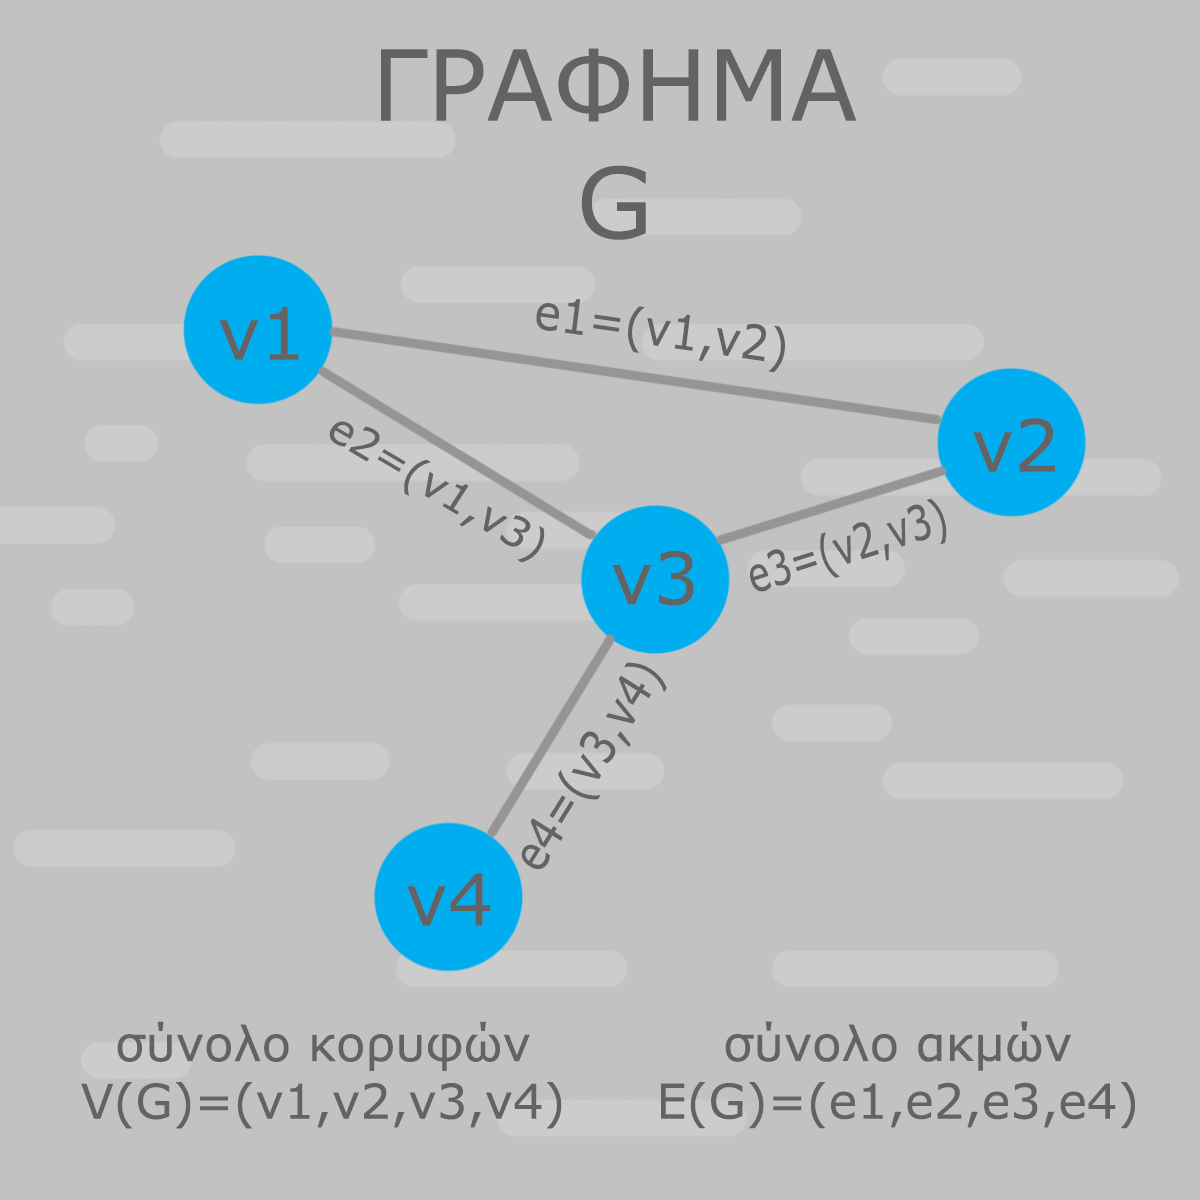
\includegraphics[scale=0.30]{2947_thesis/pictures/synola.png} 
    \caption{Σύνολα γραφήματος.}
    \label{7}
\end{figure}

Επομένως ένας γράφος είναι ένα μαθηματικό αντικείμενο που ορίζεται με αυστηρό τρόπο μέσω δύο συνόλων (sets): το σύνολο των κόρυφών (Vertices-V) και το σύνολο των ακμών (Edges-E). Το σύνολο των ακμών ενός γράφου μπορεί να είναι κενό, αυτό δεν ισχύει όμως για το σύνολο των κορυφών. \cite{Gewrgiadis2017thewria}

\subsection{Αναπαράσταση γράφων}
Την κλασσική μορφή αναπαράστασης ενός γράφου την είδαμε ήδη παραπάνω [Figure \ref{3}], όμως μια τέτοια αναπαράσταση δεν είναι καθόλου πρακτική σε προγραμματιστικό επίπεδο. Για αυτό αν θέλουμε να αναπαραστήσουμε γράφους σε έναν υπολογιστή χρησιμοποιούμε δομές δεδομένων. Οι δύο πιο βασικοί μέθοδοι αναπαράστασης γράφων σε υπολογιστές είναι οι πίνακες γειτνίασης (adjacency table) και οι λίστες γειτνίασης (adjacency lists). \footnote{Αναπαράσταση γράφων, Παναγιώτα Φατούρου, Πανεπιστήμιο Κρήτης \\link: \url{https://www.csd.uoc.gr/~hy240/current/material/teacherClasses/Section10.pdf}}

Πίνακα γειτνίασης (adjacency table) ονομάζουμε ένα πίνακα μεγέθους $nxn$, όπου $n$ ο αριθμός των κορυφών του γράφου. Κάθε κελί του πίνακα δείχνει την σχέση των αναγραφόμενων κορυφών. Σε ένα μη-κατευθυνόμενος γράφο το κελί $[i, j]$ παίρνει την τιμή 1 αν υπάρχει η ακμή $i \longleftrightarrow j$ και 0 αν δεν υπάρχει. 

Δηλαδή, έστω ο πίνακας γειτνίασης A του γράφου G:
\begin{center}
    $A[i, j] = 
    \begin{cases}
      1 & \text{αν $(i,j) \in E(G)$}\\
      0 & \text{αλλού}
    \end{cases}$
\end{center}
Είναι εύκολα αντιληπτό ότι ο πίνακας αυτός θα είναι συμμετρικός, δηλαδή ισούτε με τον ανάστροφό του, αφού η ακμή $i \longleftrightarrow j$ είναι ίδια με την ακμή $j \longleftrightarrow i$. Αντίστοιχα, σε έναν κατευθυνόμενο γράφο, το κελί $[i, j]$ παίρνει ομοίως τιμές 0 και 1 με την διαφορά ότι ο πίνακας δεν είναι συμμετρικός, οπότε η ακμή $i \rightarrow j \neq j \rightarrow i$. 

Οι πίνακες γειτνίασης μπορεί να έχουν και βάρη (weights) που είναι μια επέκταση του απλού πίνακα γειτνίασης, σε αυτήν την περίπτωση, το έκαστο κελί ενός πίνακα, αντί για 1, περιέχει έναν αριθμό που ονομάζετε βάρος και υποδηλώνει κάτι ανάλογα με την χρήση του, σε έναν αλγόριθμο βελτιστοποίησης το βάρος μπορεί να υποδηλώνει την απόσταση της μιας κορυφής από την άλλη, την πιθανότητα επιλογής αυτής της διαδρομής, την επιρροή που δέχεται κάποια οντότητα σε επόμενο πιθανό πείραμα ή οποιοδήποτε άλλο κριτήριο που ανταποκρίνεται στον σκοπό του συγκεκριμένου αλγορίθμου.
\cite{gkertsis2023thewria}
\footnote{Πίνακες γειτνίασης, Παναγιώτα Φατούρου, Πανεπιστήμιο Κρήτης \\link: \url{https://www.csd.uoc.gr/~hy240/current/material/teacherClasses/Section10.pdf}}


Για παράδειγμα στο [Figure \ref{7}], πρόκειται για έναν μη-κατευθυνόμενο γράφο χωρίς βάρη με 4 κορυφές, δηλαδή $n=4$ και με ακμές που φαίνονται στο σύνολο $E(G)$. Επομένως ο πίνακας γειτνίασης του διαμορφώνεται έτσι: 
$$
G_{n,n} = 
\begin{array}{c|c c c c}
   & v_{1} & v_{2} & v_{3} & v_{4} \\ \hline
   v_{1} & v_{1,1} & v_{1,2} & v_{1,3} & v_{1,4} \\
   v_{2} & v_{2,1} & v_{2,2} &   v_{2,3} & v_{2,4} \\
   v_{3} & v_{3,1} & v_{3,2} & v_{3,3} & v_{3,4} \\
   v_{4} & v_{4,1} & v_{4,2} & v_{4,3} & v_{4,4} 
\end{array}
$$
που αντικαθηστόντας 0-1 προκύπτει: 
$$
G_{4,4} = 
\begin{array}{c|c c c c}
   & v_{1} & v_{2} & v_{3} & v_{4} \\ \hline
   v_{1} & 0 & 1 & 1 & 0 \\
   v_{2} & 1 & 0 & 1 & 0 \\
   v_{3} & 1 & 1 & 0 & 1 \\
   v_{4} & 0 & 0 & 1 & 0 
\end{array}
$$
όπου 1 συμβολίζει ότι αυτές οι δύο κορυφές είναι γειτονικές έχοντας ακμή να τις ενώνει, ενώ 0 ότι δεν είναι. Με λίγα λόγια, αν το ζεύγος δύο κορυφών υπάρχει στο σύνολο $E(G)$ τότε το συγκεκριμένο κελί στον πίνακα γειτνίασης θα πάρει την τιμή 1, αλλιώς 0. Σε έναν τέτοιο πίνακα υπάρχει επανάληψη πληροφορίας καθώς το $v(i,j)$ είναι ίδιο με το $v(j,i)$. Σε περίπτωση κατευθυνόμενου γράφου όμως αυτό δε θα συνέβαινε αφού το κελί $v(i,j)$ θα συμβόλιζε αν υπάρχει ακμή από την κορυφή $i$ προς την κορυφή $j$, ενώ το κελί $v(j,i)$ θα συμβόλιζε αν υπάρχει ακμή από την κορυφή $j$ προς την κορυφή $i$. Σε περίπτωση ύπαρξης βαρών, τα κελιά με την τιμή 1 στον πίνακα, αντί για 1, θα είχαν την τιμή του αντίστοιχου βάρους. 

Λίστα γειτνίασης (adjacency list) ονομάζουμε μια αναπαράσταση γράφων όπου για κάθε κορυφή διατηρείται μια λίστα των γειτόνων της. Σε περίπτωση κατευθυνόμενου γράφου μπορεί να υπάρχει ξεχωριστή λίστα για τους εξερχόμενους και τους εισερχόμενους γείτονες-κορυφές. Αυτή η αναπαράσταση αποκτά αξία σε γράφους με αραιή συνδεσιμότητα αφού γίνεται εξοικονόμηση μνήμης. \footnote{Λίστες Γειτνίασης, Παναγιώτα Φατούρου, Πανεπιστήμιο Κρήτης \\link: \url{https://www.csd.uoc.gr/~hy240/current/material/teacherClasses/Section10.pdf}}

Το πόσο μεγάλη θα είναι η λίστα εξαρτάται από τον αριθμό των κορυφών του γράφου. Κάθε στοιχείο στην λίστα συμβολίζει μία ακμή του γράφου.
 
Στην περίπτωση έναν μη-κατευθυνόμενο γράφο, η λίστα γειτνίασης για κάθε κορυφή περιλαμβάνει τους γείτονές της, δηλαδή τις άλλες κορυφές με τις οποίες συνδέεται με μια ακμή. Αν υπάρχουν $n$ κορυφές στον γράφο, η λίστα γειτνίασης για κάθε κορυφή περιλαμβάνει μια λίστα με το πλήθος των γειτόνων της. Για παράδειγμα στο [Figure \ref{7}] που απεικονίζεται ένας μη-κατευθυνόμενος γράφος με 4 κορυφές, άρα $n=4$ και ακμές που φαίνονται στο σύνολο $E(G)$ του αντίστοιχου σχήματος, αν η αναπαράσταση γινόταν με λίστα γειτνίασης θα ήταν ως εξής: 
\begin{enumerate}
    \item $v1: \{v2, v3\}$
    \item $v2: \{v1, v3\}$
    \item $v3: \{v1, v2, v4\}$
    \item $v4: \{v3\}$
\end{enumerate}

Στην περίπτωση ενός κατευθυνόμενου γράφου, σε κάθε κορυφή θα υπάρχαν 2 λίστες, μία που εκφράζει τις προηγούμενες κορυφές και μία που εκφράζει τις ακόλουθες. Για παράδειγμα στο [Figure \ref{6}] η λίστα γειτνίασης θα αναπαριστόταν ως εξής: 
\begin{enumerate}
    \item Α: προηγούμενοι:$\{B, Γ\}$, ακόλουθοι:$\{B\}$
    \item Β: προηγούμενοι:$\{A, E\}$, ακόλουθοι:$\{A, E\}$
    \item Γ: προηγούμενοι:$\{E\}$, ακόλουθοι:$\{A, Z\}$
    \item Δ: προηγούμενοι:$\{Z\}$, ακόλουθοι:$\{E\}$
    \item Ε: προηγούμενοι:$\{Δ, Z\}$, ακόλουθοι:$\{B, Γ\}$
    \item Ζ: προηγούμενοι:$\{Γ\}$, ακόλουθοι:$\{Δ, E\}$
    
\end{enumerate}


Σε σχέση με τους πίνακες γειτνίασης, οι λίστες γειτνίασης επιτρέπουν την εύκολη πρόσβαση στα δεδομένα του γράφου καθώς και τροποποίηση αυτών, δηλαδή η εισαγωγή και η διαγραφή μιας κορυφής μπορεί να γίνει με ευκολία. Επίσης σε αραιούς γράφους (δηλαδή γράφους με λίγες ακμές) απαιτούν λιγότερη μνήμη, ενώ σε πλήρη συνδεδεμένους γράφους περισσότερη. 
Αντίθετα, οι πίνακες γειτνίασης δεν επιτρέπουν εύκολο τροποποίηση στις κορυφές και τις σχέσεις μεταξύ του, ούτε εύκολη εισαγωγή και διαγραφή, για παράδειγμα μία πιθανή εισαγωγή θα προκαλέσει αύξηση στο μέγεθος του πίνακα.\footnote{Θετικά και Αρνητικά, Παναγιώτα Φατούρου, Πανεπιστήμιο Κρήτης \\link: \url{https://www.csd.uoc.gr/~hy240/current/material/teacherClasses/Section10.pdf}} Όμως, το γεγονός ότι πολλές λειτουργίες μπορούν απλά και αποτελεσματικά να μοντελοποιηθούν τους κάνει ιδανικούς για χρήση στον αλγόριθμο μας. 
